\newpage
\section{Aufgabe 1}
\label{sec:a1}

\subsection{a)}
\label{subsec:a1a}
Zunächst wird für beide Populationen der Mittelwert berechnet.
\begin{align}
\mu_{P0}\approx
\begin{pmatrix*}[r]
   0,022\\
   3,026
\end{pmatrix*}\\
\mu_{P1}\approx
\begin{pmatrix*}[r]
   5,986\\
   3,026
\end{pmatrix*}
\end{align}

\subsection{b)}
\label{subsec:a1b}
Die Kovantianzmatrix $S_{P0}$ und $S_{P1}$ berechnen sich über
\begin{align}
S_j=\sum_i^{n_j}(\vec x- \vec \mu_j)(\vec x- \vec \mu_j)^T
\intertext{zu}
S_{P0}\approx
\begin{pmatrix*}[r]
     122904 &  81979\\
     81979  &  67449
\end{pmatrix*}
\intertext{und}
S_{P1}\approx
\begin{pmatrix*}[r]
    122344 &  73118\\
     73118 &   53845
\end{pmatrix*}
\intertext{Aus $S_{P0P1}=S_{P0}+S_{P1}$ folgt}
S_{P0P1}\approx
\begin{pmatrix*}[r]
 245248  & 155097\\
 155097  & 121294
\end{pmatrix*}
\intertext{Desweiteren muss noch $S_B$ über}
S_B=(\vec \mu_1-\vec \mu_2)(\vec \mu_1-\vec \mu_2)^T
\intertext{berechnet werden.}
\Rightarrow S_B\approx
\begin{pmatrix*}[r]
 35.562 &   0.432\\
 0.432  & 0.005
\end{pmatrix*}
\end{align}

\subsection{c)}
\label{subsec:a1c}

Um nun die Fisher-Diskriminate zu berechen, müssen
die Eigenwerte und Eigenvektoren der Matrix
\begin{align}
A=S_{P0P1}^{-1}S_B
\end{align}
berechnet werden.
Die Inverse von $S_{P0P1}$ lautet:
\begin{align}
  S_{P0P1}^{-1}\approx&
  \begin{pmatrix*}[r]
   0.000021 & -0.000027 \\
  -0.000027 &  0.000043
  \end{pmatrix*}
\intertext{somit folgt für $A$}
A\approx&
\begin{pmatrix*}[r]
 0.000746 &  0.000009 \\
-0.000950 & -0.000012
\end{pmatrix*}
\intertext{Die Eigenwerte der Matrix $A$ sind:}
\lambda_1\approx&0,0007   \qquad \lambda_2\approx0
\intertext{Die normierten Eigenvektoren sind:}
\vec v_{\lambda_1}\approx&
\begin{pmatrix*}[r]
 0,617\\
 -0,012
\end{pmatrix*}\\
\vec v_{\lambda_2}\approx&
\begin{pmatrix*}[r]
-0,787\\
1
\end{pmatrix*}
\intertext{Als Projektionsvektors wird der
 Eigenvektor zum Eigenwert $\lambda_1$ gewählt.
 Daraus folgt die Geradengleichung:}
\vec \lambda =\lambda \cdot
\begin{pmatrix*}[r]
 0,617\\
 -0,012
\end{pmatrix*}
\end{align}
\subsection{d)}
\label{subsec:a1d}
Nun kann mit Hilfe des Projektionsvektors
ein eindimensionales Histogramm der Populationen \ref{fig:hist} berechnete werden.
\begin{figure}
  \centering
  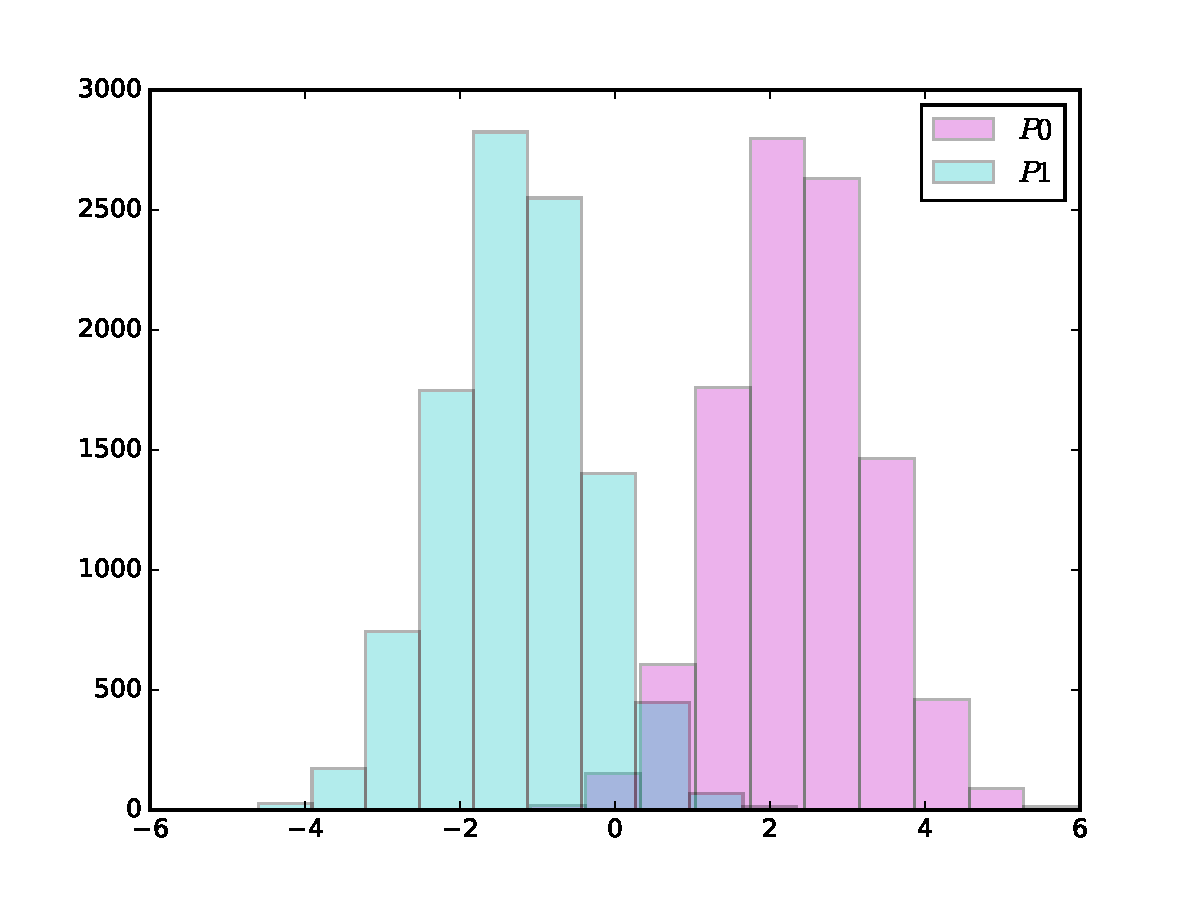
\includegraphics[width=0.7\textwidth]{Projektion.pdf}
  \caption{Histogramm der Projektion
   von den Populationen
   $P0$ und $P1$ auf die Projektionsgeraden $\vec\lambda$.}
  \label{fig:hist}
\end{figure}
\FloatBarrier

\subsection{e)}
\label{subsec:a1e}
Betrachtet man nun $P0$ als Signal und $P1$ als Untergrund kann die
Effizienz und Reinheit des Signals als Funktion eines Schnitts
$\lambda_\mathrm{cut}$ aufgetragen werden.
Der folgende Potts \ref{fig:cut}
dargestellt.

\begin{figure}
  \centering
  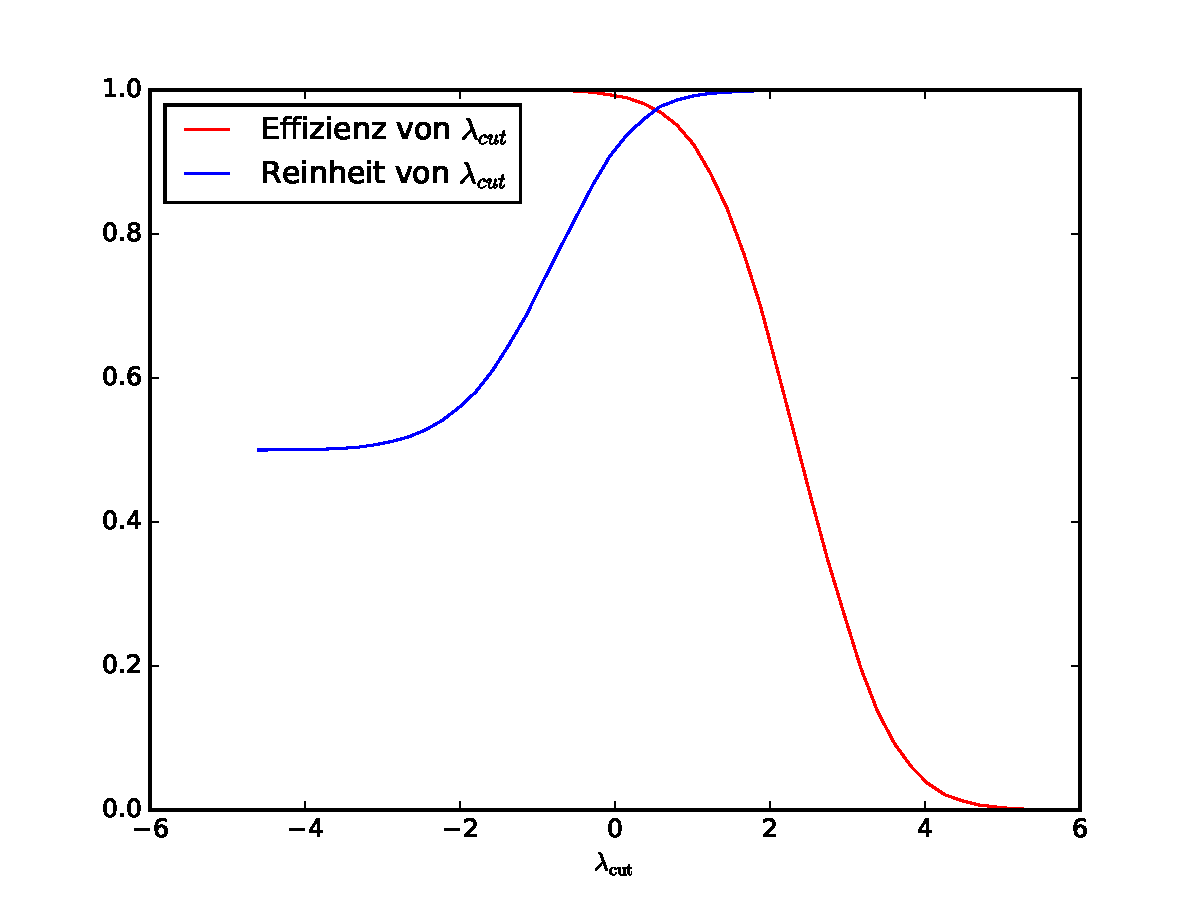
\includegraphics[width=0.7\textwidth]{Eff_Rein.pdf}
  \caption{Effizienz und Reinheit des Schnittes ausgehend von der Gerade $\vec \lambda$ in Abhängigkeit von $\lambda_\text{cut}$ .}
  \label{fig:cut1}
\end{figure}

\FloatBarrier

\subsection{f)}
\label{subsec:a1f}

\subsection{g)}
\label{subsec:a1g}

\subsection{h)}
\label{subsec:a1h}
